\documentclass{article}

\usepackage{geometry}
\usepackage{amsmath}
\usepackage{graphicx}
\usepackage{listings}
\usepackage{hyperref}
\usepackage{multicol}
\usepackage{fancyhdr}
\pagestyle{fancy}
\hypersetup{ colorlinks=true, linkcolor=black, filecolor=magenta, urlcolor=cyan}
\geometry{ a4paper, total={170mm,257mm}, top=20mm, right=20mm, bottom=20mm, left=20mm}
\setlength{\parindent}{0pt}
\setlength{\parskip}{1em}
\renewcommand{\headrulewidth}{0pt}
\lhead{Competitive Programming - ITB}
\fancyfoot[CE,CO]{\thepage}
\lstset{
    basicstyle=\ttfamily\small,
    columns=fixed,
    extendedchars=true,
    breaklines=true,
    tabsize=2,
    prebreak=\raisebox{0ex}[0ex][0ex]{\ensuremath{\hookleftarrow}},
    frame=none,
    showtabs=false,
    showspaces=false,
    showstringspaces=false,
    prebreak={},
    keywordstyle=\color[rgb]{0.627,0.126,0.941},
    commentstyle=\color[rgb]{0.133,0.545,0.133},
    stringstyle=\color[rgb]{01,0,0},
    captionpos=t,
    escapeinside={(\%}{\%)}
}

\begin{document}

\begin{center}
    \section*{Cegah Penyebaran Corona} % ganti judul soal

    \begin{tabular}{ | c c | }
        \hline
        Batas Waktu  & 1s \\    % jangan lupa ganti time limit
        Batas Memori & 512MB \\  % jangan lupa ganti memory limit
        \hline
    \end{tabular}
\end{center}

\subsection*{Deskripsi}

Di sebuah galaksi jauh jauh disana (sebut saja Galaksi Stonks), sedang terjadi pandemi Coronavirus! Pemerintah telah meminta semua penduduknya untuk berdiam di rumah dan mencegah persebaran virus. Akan tetapi, mereka malah pergi liburan ke luar rumah. Virus menyebar dan menginfeksi orang - orang dengan sangat cepat. Untungnya, ada seorang peneliti biologi handal yang bernama Mufraswid. Dia telah membuat peta persebaran Coronavirus. Ternyata, setiap orang menyebarkan virus ini ke \underline{tepat} $k$ orang lain. Selain itu, virus ini akan hilang dengan sendirinya setelah menginfeksi semua orang dengan generasi ke - $h$.
\par
Untungnya ada $n$ orang yang menuruti perkataan pemerintah dan bermain Dota 2 di rumahnya. Orang - orang yang diam di rumah tidak akan menyebar Coronavirus kepada orang lain. Mufraswid penasaran, berapa banyak orang yang terinfeksi Coronavirus di Galaksi Stonks? Karena bilangan bisa bernilai sangat besar, keluarkan nilai tersebut modulo $10^9 + 7$.
\par
Penduduk di Galaksi Stonks dinomori dengan aturan sebagai berikut:
\begin{enumerate}
    \setlength\itemsep{0pt}
    \item Patient zero memiliki nomor $0$.
    \item Generasi ke - $1$ memiliki nomor $1, 2, ..., k$.
    \item Generasi ke - $2$ memiliki nomor $k+1, k+2, ..., k+k*k$.
    dan seterusnya
\end{enumerate}
\par
Sebagai contoh, lihat pohon dengan nilai $k = 2$ dan $h = 4$. Misalkan penduduk yang bernomor $2$, $4$ dan $5$ memutuskan untuk tidak keluar rumah:
\begin{center}
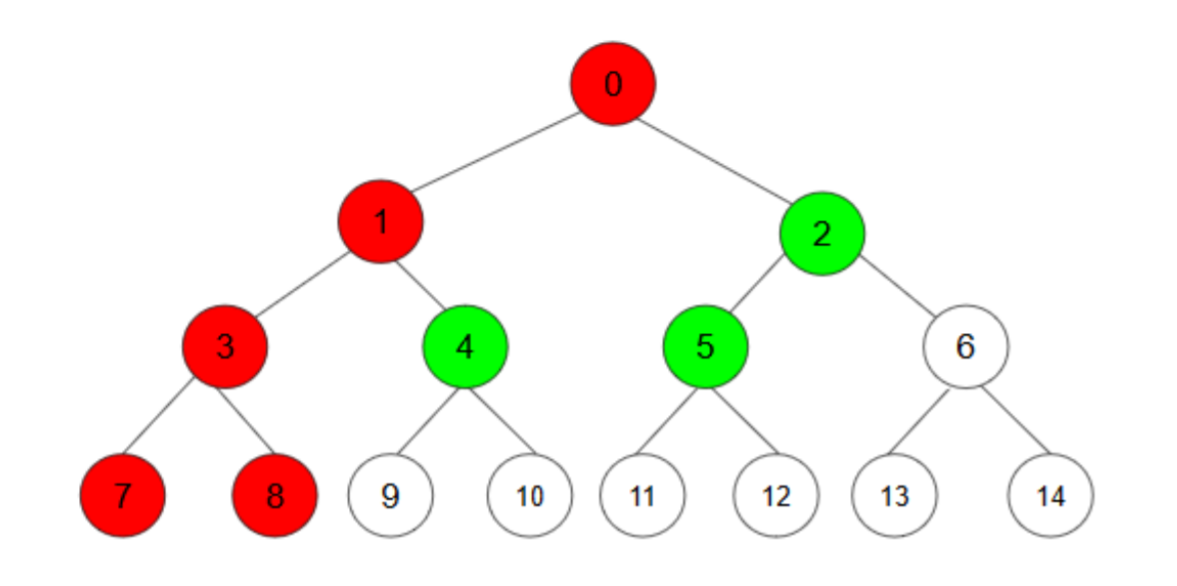
\includegraphics[scale=0.6]{tree}
\end{center}
Node menandakan penduduk Galaksi Stonks. Node merah menandakan penduduk yang terinfeksi. Node hijau menandakan penduduk yang tetap di rumah dan tidak terinfeksi. Node putih adalah penduduk yang tidak terinfeksi.
\par
Dari contoh diatas, terlihat bahwa ada 5 orang yang terinfeksi Coronavirus. Orang yang tidak keluar rumah telah mencegah persebaran virus ini.
\pagebreak

\subsection*{Format Masukan}

Baris pertama terdiri dari tiga bilangan bulat positif $k$, $h$ dan $n$. $k$ menyatakan banyaknya orang yang bisa disebarkan 1 orang. $h$ menyatakan banyaknya generasi sebelum virus hilang. $n$ menyatakan banyaknya penduduk yang tidak keluar rumah.
\par
Baris kedua terdiri dari $n$ bilangan, yang menyatakan nomor penduduk yang tidak keluar rumah.

\subsection*{Format Keluaran}

1 buah bilangan, yang menyatakan banyaknya orang yang terinfeksi Coronavirus modulo $10^9+7$

\subsection*{Batasan}

\begin{itemize}
    \setlength\itemsep{0pt}
    \item $1 \leq k, h, n \leq 10^5$
    \item $0 \leq $ semua elemen $n \leq 10^{12}$, dijamin valid
\end{itemize}

\begin{multicols}{2}
\subsection*{Contoh Masukan}
\begin{lstlisting}
2 4 3
2 5 4
\end{lstlisting}
\columnbreak
\subsection*{Contoh Keluaran}
\begin{lstlisting}
5
\end{lstlisting}
\vfill
\null
\end{multicols}

\begin{multicols}{2}
\subsection*{Contoh Masukan}
\begin{lstlisting}
3 4 6
2 6 12 26 10 36
\end{lstlisting}
\columnbreak
\subsection*{Contoh Keluaran}
\begin{lstlisting}
10
\end{lstlisting}
\vfill
\null
\end{multicols}
% \subsection*{Penjelasan}
% Jika dibutuhkan, tambahkan penjelasan di sini

\pagebreak

\end{document}